\documentclass[letter]{article}
\renewcommand{\baselinestretch}{1.25}

\usepackage[margin=1in]{geometry}
\usepackage{physics}
\usepackage{amsmath}
\usepackage{graphicx}
%\usepackage{pythonhighlight}
\usepackage{hyperref}
\usepackage{fancyvrb}


% MATLAB Formating Code
\usepackage[numbered,framed]{matlab-prettifier}
\lstset{style=Matlab-editor,columns=fullflexible}
\renewcommand{\lstlistingname}{Script}
\newcommand{\scriptname}{\lstlistingname}

% Command for easier minimization problem def
\newcommand{\optpblm}[3][eq:default]{
	\begin{equation}\label{#1}
% Array method... more centered		
%		\begin{array}{rl}
%			\text{minimize}  \hspace{0.2in} &#2 \vspace{5pt}\\
%			\text{subject to} \hspace{0.2in} &#3
%		\end{array}
% Aligned method... left aligned... idk if its better
		\begin{aligned}
			\text{minimize} \hspace{0.5in} &#2\vspace{5pt}\\
			\text{subject to \hspace{0.5in}} &#3
		\end{aligned}	
	\end{equation}
}



\allowdisplaybreaks

%opening
\title{MECH 6327 - Homework 3}
\author{Jonas Wagner}
\date{2021, March 24}

\begin{document}

\maketitle

\newpage
%\textbf{(Probably not necessary... but its long)}
\tableofcontents

\newpage
\section*{BV Textobook Problems}
\subsection{Problem 4.11}
\textbf{Problem:}
Formulate each problem as a LP and explained the relationship between the optimal solution of the problems and the solution of its LP.\\
\textbf{Solution:}
\subsubsection{Part a: Minimize $\norm{Ax-b}_\infty$}
Define the following minimization problem:
\optpblm{\norm{Ax-b}_\infty}{\text{math}}
From the definition of an $\infty$-norm as $$\norm{x}_\infty = \max_i \abs{x_i}$$ the following can be derived:
\optpblm{t}{\qty(Ax - b)_i\leq t, \ \forall i = 1,\dots,n\\
		- & \qty(Ax - b)_i\leq t, \ \forall i = 1,\dots,n}
Which is equivalent to the following linear program
\optpblm{t}{-\vb{1}t \leq Ax - b \leq \vb{1}t}
This minimum is related to the original minimization problem by the following transformation:
****************************************** fill in details


\newpage
\subsubsection{Part b: Minimize $\norm{Ax-b}_1$}
Define the following minimization problem:
\optpblm{\norm{Ax-b}_1}{\text{math}}
From the definition of an $1$-norm as $$\norm{x}_1 = \sum_i \abs{x_i}$$ the following can be derived:
\optpblm{t_1 + \cdots + t_n}{\qty(Ax - b)_i\leq t_i, \ \forall i = 1,\dots,n\\
-	& \qty(Ax - b)_i\leq t_i, \ \forall i = 1,\dots,n}
Which is equivalent to the following linear program
\optpblm{\vb{1}^T t}{-t \leq Ax - b \leq t}

This minimum is related to the original minimization problem by the following transformation:


****************************************** fill in details

\newpage
\subsubsection{Part c: Minimize $\norm{Ax-b}_1$ subject to $\norm{x}_{\infty}\leq 1$}
Define the following minimization problem:
\optpblm{\norm{Ax-b}_1}{\norm{x}_\infty \leq 1}
From the definition of an $1$-norm as $$\norm{x}_1 = \sum_i \abs{x_i}$$ and the definition of an $\infty$-norm as $$\norm{x}_\infty = \max_i \abs{x_i}$$ the following can be derived:
\optpblm{t_1 + \cdots + t_n}{\qty(Ax - b)_i\leq t_i, \ \forall i = 1,\dots,n\\
	-& \qty(Ax - b)_i\leq t_i, \ \forall i = 1,\dots,n\\
	 & x_i \leq 1, \forall i = 1,\dots,n\\
	-& x_i \leq 1, \forall i = 1,\dots,n}
Which is equivalent to the following linear program
\optpblm{\vb{1}^T t}{-t \leq Ax - b \leq t\\
					&-\vb{1} \leq x \leq \vb{1}}
%				&-1 \leq x_i \leq 1, \ \forall i = 1,\dots,n}
This minimum is related to the original minimization problem by the following transformation:

****************************************** fill in details

\newpage
\subsubsection{Part d: Minimize $\norm{x}_1$ subject to $\norm{Ax-b}_\infty \leq 1$}
Define the following minimization problem:
\optpblm{\norm{x}_1}{\norm{Ax-b}_\infty \leq 1}
From the definition of an $1$-norm as $$\norm{x}_1 = \sum_i \abs{x_i}$$ and the definition of an $\infty$-norm as $$\norm{x}_\infty = \max_i \abs{x_i}$$ the following can be derived:
\optpblm{t_1 + \cdots + t_n}{x_i \leq t_i, \ \forall i = 1,\dots,n\\
							&-x_i \leq t_i, \ \forall i = 1,\dots,n\\
							&(Ax-b)_i \leq 1, \ \forall i = 1,\dots,n}
From this a linear program can be defined as:
\optpblm{\vb{1}^T t}{-t \leq x \leq t\\
			 		&Ax - b \leq \vb{1}}
This minimum is related to the original minimization problem by the following transformation:

****************************************** fill in details

\newpage
\subsubsection{Part e: Minimize $\norm{Ax-b}_1 + \norm{x}_\infty$}
Define the following minimization problem:
\optpblm{\norm{Ax-b}_1 + \norm{x}_\infty}{math}
From the definition of an $1$-norm as $$\norm{x}_1 = \sum_i \abs{x_i}$$ and the definition of an $\infty$-norm as $$\norm{x}_\infty = \max_i \abs{x_i}$$ the following can be derived:
\optpblm{t_1 + \cdots + t_n + s}{
		\qty(Ax - b)_i\leq t_i, \ \forall i = 1,\dots,n\\
		-& \qty(Ax - b)_i\leq t_i, \ \forall i = 1,\dots,n\\
		&x_i \leq s, \ \forall i = 1,\dots,n\\
	-	&x_i \leq s, \ \forall i = 1,\dots,n}
This can be written as a standard linear program as:
\optpblm{\vb{1}^T t + s}{
		- t \leq Ax-b \leq t\\
		&-\vb{1}s \leq x \leq \vb{1}s}
This minimum is related to the original minimization problem by the following transformation:

****************************************** fill in details

\newpage
\subsection{Problem 4.16}
Consider the system given as
\begin{equation}\label{eq:dyn_sys_def}
	x(t+1) = A x(t) + b u(t), \ t = 0,\dots,N-1
\end{equation}
with $x(t) \in \real^n, u(t) \in \real, \forall t = 0,\dots,N-1$ and $A \in \real^{n\cross n}, b \in \real^n$, and $x(0) = 0$.\\

The minimum fuel optimal control problem is to select the minimum amount of inputs to minimize the amount of fuel used, given as
\begin{equation}\label{eq:min_fuel_problem_def}
	\begin{aligned}
		\text{minimize} \hspace{0.5in} &F = \sum_{t=1}^{N-1} f(u(t))\\
		\text{subject to \hspace{0.5in}} & x(t+1) = A x(t) + b u(t), \ t = 0,\dots,N-1\\
		& x(N) = x_{des}
	\end{aligned}	
\end{equation}
with $N$ as the time-horizon, $x_{des} \in \real^n$ as the desired final state, and $f: \real \to \real$ given as
\begin{equation}\label{eq:fuel_usage_def}
	f(a) = 
	\begin{cases}
		\abs{a} & \abs{a} \leq 1 \\
		2 \abs{a} - 1 & \abs{a} > 1
	\end{cases}
\end{equation}

\textbf{Problem:}
Formulate this problem as a Linear Program.\\

\textbf{Solution:}
First, \ref{eq:min_fuel_problem_def} can be rewritten in an epigraph form (with the additional assumption that $f(u(t))$ is always positive):
\optpblm[eq:min_fuel_problem_epigraph]{F_1 + \cdots + F_{N-1}}{
		f(u(t)) = F_t, \ \forall t = 1, \dots, N-1\\
		& x(t+1) = A x(t) + b u(t), \ \forall t = 0,\dots,N-1\\
		&x(N) = x_{des}}
Now looking at the nonlinear component, fuel usage as defined by \eqref{eq:fuel_usage_def}, can be equated to:
\begin{equation}
	\begin{aligned}
		\abs{a} \leq g\\
		2 \abs{a} - 1 \leq g\\
	\end{aligned}
\end{equation}
or equivalently,
\begin{equation}
	\begin{aligned}
		-g \leq a \leq g\\
		-g \leq 2a -1 \leq g
	\end{aligned}
\end{equation}

This represents an intersection of two half-spaces which is a simpliler convex restriction.\\
This can now be combined with \eqref{eq:min_fuel_problem_epigraph} to produce the linear program:
\optpblm[eq:min_fuel_problem_result]{F_1 + \cdots + F_{N-1}}{
	-F_t \leq u(t) \leq F_t, \ \forall t = 1, \dots, N-1\\
	&-F_t \leq 2u(t) -1 \leq F_t, \ \forall t = 1, \dots, N-1\\
	& x(t+1) = A x(t) + b u(t), \ \forall t = 0,\dots,N-1\\
	&x(N) = x_{des}}
Which can then be rewritten as:
\optpblm[eq:min_fuel_problem_result]{\vb{1}^T F}{
		-F \leq \vb{u} \leq F\\
		& x(t+1) = A x(t) + b u(t), \ \forall t = 0,\dots,N-1\\
		&x(N) = x_{des}}


\newpage
\subsection{Problem 4.28}
Consider the convex quadratic program given as
\begin{equation}\label{eq:convex_quadratic_program}
	\begin{aligned}
		\text{minimize} \ \ & \frac{1}{2} x^T P x + q^T x + r\\
		\text{subject to} \ \ & Ax \preceq b
	\end{aligned}
\end{equation}
with a robust equivalent defined as
\begin{equation}\label{eq:robust_convex_quadratic_program}
	\begin{aligned}
		\text{minimize} \ \ & \sup_{P\in \mathcal{E}}{\frac{1}{2} x^T P x + q^T x + r}\\
		\text{subject to} \ \ & Ax \preceq b
	\end{aligned}
\end{equation}
where $\mathcal{E}$ is the set of all possible matrices of $P$.

\subsubsection{Part a}
\textbf{Problem:}
Express the robust QP as a convex problem given $\mathcal{E} = {P_1,\dots,P_k}$ where $P_i\in S^n_+, i = 1,\dots,K$.\\

\textbf{Solution:}





% no part b,c for 4.28


\newpage
\subsection{Problem 4.43}
Suppose $A: \real^n \to S^m$ is affine such that
\begin{equation}
	A(x) = A_0 + x_1 A_1 + \cdots + x_n A_n
\end{equation}
where $A_i \in S^m$. Let $\lambda_1(x) \geq \lambda_2(x) \geq \cdots \geq \lambda_m(x)$ be the eigenvalues of $A(x)$.\\


For each of the following minimization criteria, formulate the problem as an SDP.\\

\subsubsection{Part a}
\textbf{Problem:}
Minimize the maximum eigenvalue of $A$: $$\text{minimize} \ \ \lambda_1(x)$$\\
\textbf{Solution:}





\subsubsection{Part b}
\textbf{Problem:}
Minimize the spread of the eigenvalues of $A$: $$\text{minimize} \ \ \lambda_1(x) - \lambda_m(x)$$\\
\textbf{Solution:}










\subsubsection{Part c}
\textbf{Problem:}
Minimize the conditional number of $A$ while remaining postive definite:
\begin{equation*}
	\begin{aligned}
		\text{minimize} \ \ &k(A(x)) = \frac{\lambda_1(x)}{\lambda_m(x)} \ \forall \ x \in \{x \ | \ A(x) \succ 0\}\\
		 \text{subject to} \ \ &A(x) \succ 0
	\end{aligned}
\end{equation*}
\textbf{Solution:}








% Only Part a,b,c for 4.43






\newpage
\section{Problem 1: Open-loop optimal control with $1-$ and $\infty-$ norms.}
The following open-loop optimal regulation problem is given as:
\begin{equation}\label{eq:open-loop_opt-control_def}
	\begin{aligned}
		\text{minimze} \hspace{0.5in}&\norm{x_T}_p + \sum_{t = 0}^{T-1} \norm{x_t}_p + \gamma\norm{u_t}_q\\
		\text{subject to} \hspace{0.5in} 	& x_{t+1} = A x_t + B u_t, \ t = 0,\dots,T-1\\
							& \norm{x_t}_\infty \leq \bar{x}, \ t = 0,\dots,T\\
							 & \norm{u_t}_\infty \leq \bar{u}, \ t = 0,\dots,T
	\end{aligned}
\end{equation}
with $x_t \in \real^n$ and $u_t \in \real^m$ as the system state and control input respectively and parameter $\gamma > 0$ governing the actuator and state regulation performance.\\

\textbf{Problem:}
Express this problem as a linear program for (i) $p=q=\infty$ and (ii) $p=q=1$. Code both in CVX and for the problem data provided. Verify the equivalence between the original optimization problem and transformed linear program obtained and plot the optimal state and input trajectories for each.\\

\textbf{Solution:}
\subsection{Linear program for $p = q = \infty$}





\subsection{Linear program for $p = q = 1$}





\subsection{CVX Formulation and Results:}












\newpage
\section{Problem 2: Minimum time state transfer via quasiconvex optimization.}
Consider the LTI system:
\begin{equation}\label{eq:quasiconvex_opt_def}
	x_{t+1} = Ax_t + B u_t, \ t = 0,\dots,T\\
	\underline{u} \leq u_t \leq \bar{u}, t = 0,\dots,T
\end{equation}
with $x_0$ as the initial state.

\textbf{Problem:}
Show that the minimum time required to transfer the system from $x_0$ to $x_{desired}$, given as
\begin{equation}\label{eq:qualiconvex_problem_result}
	f(u_0,\dots,u_T) = \min{\tau \ | \ x_t = x_{desired} \text{for} \tau \leq t \leq {T+1}}
\end{equation}
is a quasiconvex function. Impliment a bisection algorithm to solve the problem for the given data.

\textbf{Solution:}








\newpage
\section{Problem 3: State feedback control design via SDP}
Feedback control problems can be formulated using a semidefinite program, such as
\begin{equation}\label{eq:feedback_control_def}
	\begin{aligned}
		\text{minimze} \hspace{0.5in}& \trace{P}
		\text{subject to} \hspace{0.5in}
		& \mqty [R + B^T PB & B^T PA\\
				 A^T PB & Q + A^T P A - P] \succeq 0\\
				 & P \succeq 0
	\end{aligned}
\end{equation}
with variable $P \in S^n$ and problem data $A\in \real^{n\cross n}, B \in\real^{n\cross m}, Q \in S^n_+, \real \in S^m_{++}$.\\

This problem is equivalent to the solution to the optimal solution to the infinite-horizon LQR problem:
\begin{equation}\label{eq:LQR_control_def}
	\begin{aligned}
		\text{minimze} \hspace{0.5in}& \sum_{t=0}^\infty x_t^T Q x_t + u_t^T R u_t
		\text{subject to} \hspace{0.5in}
		& x_{t+1} = Ax_t + B u_t, \ t \geq 0, \ x(t=0) = x_0
	\end{aligned}
\end{equation}
This is also equivelent to the solution the the discrete-time richotte equation (DARE) and can be solved in matlab with dare(A,B,Q,R). The solution to the feedback controller is
\begin{equation}\label{eq:LQR_control_solution}
	u_t = K x_t\\
	K = -\qty(R + B^T B)^{-1} B^T P^* A
\end{equation}

\textbf{Problem:}
Confirm the solution to the SDP given in \eqref{eq:feedback_control_def} is equivalent to the LQR problem given in \eqref{eq:LQR_control_def} for multiple randomly generated problems.

\textbf{Solution:}
The following results are provided for various randomly generated problems and solutions. This was generated using the code in \appendixname \ref{apx:pblm3_matlab}.

\begin{Verbatim}
	contents....
\end{Verbatim}















\newpage
\appendix
\section{MATLAB Code:}\label{apx:matlab}
All code I write in this course can be found on my GitHub repository:\\
\href{https://github.com/jonaswagner2826/MECH6313}{https://github.com/jonaswagner2826/MECH6327}
%\lstinputlisting[caption={MECH6323\_HW3},label={script:HW1}]{MECH6327_HW3.m}


\newpage
\section{Problem 3 MATLAB Code:}\label{apx:pblm3_matlab}
All code I write in this course can be found on my GitHub repository:\\
\href{https://github.com/jonaswagner2826/MECH6313}{https://github.com/jonaswagner2826/MECH6327}
% MECH6313_HW3
%\lstinputlisting[caption={MECH6323\_HW3},label={script:HW1}]{MECH6327_HW3_pblm3.m}















%--------------------------------------------- HW2
%\section{Problem Set 1: Convex Sets}
%
%\subsection{Problem 2.5}
%\textbf{Problem:}\\
%What is the distance between two parallel hyperplanes: $\{x \in \real^n | a^T x = b_1\}$ and $\{x \in \real^n | a^T x = b_2\}$?\\
%
%\noindent
%\textbf{Solution:}\\
%Under the assumption that $a\in \real^n$ and $b_1,b_2 \in \real$, the quantity $a^T x_0$ represents the component of $x_0$ in the normal direction. Similarly, the quantities $b_1$ and $b_2$ represent the euclidean distance of the hyperplane from the origin (in the normal direction). Since the hyperplanes are parrellel, the distance between them is the difference between their offsets:
%\begin{equation}
%	\text{Distance between hyperplanes: } b_1 - b_2
%\end{equation}
%
%
%\subsection{Problem 2.7}
%\textbf{Problem:}\\
%\textit{Voronoi description of halfspace.} Let $a$ and $b$ be distinct points in $\real^n$. Show that the set of all points that are closer to $a$ than $b$ via the euclidean norm is a halfspace. Describe it explicitly as an inequality and draw a picture.
%
%\noindent
%\textbf{Solution:}\\
%The set of all points closer to $a$ then $b$ can be defined as:
%\begin{equation}
%	\{x \in \real^n \ | \ \norm{x-a}_2 \leq \norm{x-b}_2\}
%\end{equation}
%
%The boundary defining this halfspace will be a plane defined by the normal vector $c$ representing the distance between $a$ and $b$, and the offset coefficient $d$ describing intersection of the plane through the half-way point between $a$ and $b$. The quantities $c$ and $d$ can therefore be defined by:
%\begin{equation}
%	\begin{aligned}
%		c &= b - a\\
%		d &= \frac{c^T a + c^T b}{2}\\
%		  &= \frac{1}{2} c^T (a+b)
%	\end{aligned}
%\end{equation}
%
%The halfspace, that is equivalent to $x$, can be described by the following:
%\begin{equation}
%	\{x\in \real^n \ | \ c^T x \leq d\}
%\end{equation}
%
%This can be visualized in two dimensions for $a = \mqty[2\\4]$ and $b = \mqty[-3\\7]$. The boundary (the red line) is calculated in the standard form using $$x_2 = \frac{-1}{c_2} \qty(c_1 * x_1 - d)$$ and then plotted. The half-space itself is the region below the boundary.
%%
%%\begin{figure}[h]
%%	\centering
%%	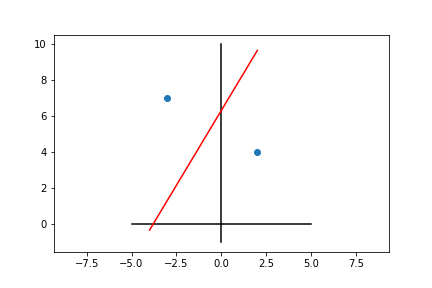
\includegraphics[width = 0.7\linewidth]{fig/pblm2_7}
%%	\caption{Visualization of the boundary for the halfspace.}
%%	\label{fig:pblm2_7}
%%\end{figure}
%
%
%%\newpage
%\subsection{Problem 2.12}
%\textbf{Problem:}\\
%Which of the following sets are convex?\\
%
%\noindent
%\textbf{Solution:}
%\subsubsection{(a) - Slab}
%A slab defined as $$\{x \in \real^n \ | \ \alpha \leq a^T x \leq \beta\}$$ \textbf{is convex} as it consists of the intersection of two halfspaces which themselves are complex.
%
%\subsubsection{(b) - Rectangle/Hyperrectangle}
%A rectangle set defined as $$\{x \in \real^n \ | \ \alpha_i \leq x_i \leq \beta_i, \ i = 1,\dots,n\}$$ \textbf{is convex} as it is composed of the intersections of half spaces which are themselves convex. This is similar to the polyhedrons/polytopes that by definition are also convex.
%
%\subsubsection{(c) - Wedge}
%A wedge set given as $$\{x \in \real^n \ | \ a_1^T x \leq b_1, a_2^T x \leq b_2\}$$ \textbf{is convex} as it is just an intersection of two halfspaces (a polyhedron).
%
%\subsubsection{(d) - Closer to a point then a set}
%A set of points closer to a given point than a given set is defined as $$\{x \| \norm{x-x_0}_2 \leq \norm{x - y}_2 \ \forall y \in S\}$$ where $S\subset\real^n$ \textbf{is not convex} in general. This is because there is not enough information about $y$ for a conclusion to be made whether it is convex or not. A counter example would be if $y$ is a point in orbit around a convex shape $S$ that would end up generating a concave $x$.
%
%\subsubsection{(e) - Closer to a set then another set}
%A set of points closer to a given set than another given set is defined as $$\{x \ | \ \textbf{dist}(x,S) \leq \textbf{dist}(x,T)\}$$ where $S, T \subset\real^n$, and $$\textbf{dist}(x,S) = \inf\{\norm{x-z}_2 \ | \ z \in S\}$$ \textbf{is not convex} in general. This is because there is not enough information about $S$ and $T$ for a conclusion to be made whether it is convex or not. A counter example includes if $S$ or $T$ themselves are a concave shave that causes the set $x$ to also be concave and therefore not convex.
%
%
%\subsubsection{(f) - Set of the sum being within a convex set}
%The set defined as $$\{x \ | \ x + S_2 \subseteq S_1\}$$ with $S_1$ being convex \textbf{is not complex} in general. This is because we do not know enough information about $S_2$ to conclude that $x$ is conncex purely due to the relationship with the convex set $S_1$.\\
%
%\subsubsection{(g) - Set with weighted distances to two points}
%The set of all points that is closer to $a$ then $b$ by at least a factor of $\theta$, defined as $$\{x \in \real^n \ | \ \norm{x-a}_2 \leq \theta \norm{x-b}_2\}$$ with $a \neq b$ and $0 \leq \theta \leq 1$ \textbf{is convex.} This is know because, as proven in a previous problem, a hyperplane is formed for a similarity stated problem which itself is convex. When the distance to $a$ must be less then a portion of the distance to $b$ it will cause the psudo-hyperplane to curve inwards and untimely remain convex.
%
%
%\newpage
%\subsection{Problem 2.28}
%\textbf{Problem:}\\
%Define the positive semi-definite cone ($S_+^n$) for $n = 1, 2, 3$ in terms of ordinary inequalities with the matrix coefficients themselves.
%
%\noindent
%\textbf{Solution:}\\
%The positive semi-definite cone is defined for size $n$ as the set of all symmetric matrices that are positive semi-definite:
%\begin{equation}
%	S_+^n \equiv \{x \in S^n \ | \ x \succeq 0\}
%\end{equation}
%One method to ensure that a matrix is positive semi-definite is to ensure that its leading principle minors are all non-negative (strictly positive for positive definite).\\
%
%For $n=1$ the required inequalities are simple, 
%\begin{equation}
%	X = \mqty[x_1] \in S_+^1 \iff x_1 \geq 0
%\end{equation}
%
%For $n=2$ the inequalities can be found by ensuring the leading principle minors are all non negative:
%\begin{equation}
%	\begin{aligned}
%		m_1 &= \det[x_1]\\
%		&= x_1\\
%		m_2 &= \det \mqty[x_1 & x_2 \\ x_2 & x_3] \\
%		&= x_1 x_3 - x_2^2
%	\end{aligned}
%\end{equation}
%These definitions of the minors can be then be used to construct inequalities such that all the minors are positive:
%\begin{equation}
%	X = \mqty[x_1 & x_2 \\ x_2 & x_3] \in S_+^2 \ \iff \ \mqty{x_1 \geq 0\\  x_1 x_3 \geq x_2^2}
%\end{equation}
%
%For $n=3$ the inequalities can be found by ensuring the leading principle minors are all non negative:
%\begin{equation}
%	\begin{aligned}
%		m_1 &= \det[x_1]\\
%		&= x_1\\
%		m_2 &= \det \mqty[x_1 & x_2 \\ x_2 & x_4] \\
%		&= x_1 x_4 - x_2^2\\
%		m_3 &= \det \mqty[x_1 & x_2 & x_3\\ x_2 & x_4 & x_5\\ x_3 & x_5 & x_6]\\
%		&= x_1 (x_1 x_4 - x_2^2) - x_2 (x_2 x_6 - x_3 x_5) + x_3 (x_2 x_5 - x_3 x_4)\\
%		&= x_1^2 x_4 - x_1 x_2^2 - x_2^2 x_6 + x_2 x_3 x_5 + x_2 x_3 x_5 - x_3^2 x_4
%	\end{aligned}
%\end{equation}
%These definitions of the minors can be then be used to construct inequalities such that all the minors are positive:
%\begin{equation}
%	X = \mqty[x_1 & x_2 & x_3\\ x_2 & x_4 & x_5\\ x_3 & x_5 & x_6] \in S_+^2 \ \iff \ 
%	\mqty{x_1 \geq 0\\
%			x_1 x_4 \geq x_2^2\\
%		 x_1 x_2^2 + x_2^2 x_6 + x_3^2 x_4 \geq x_1^2 x_4 + 2 x_2 x_3 x_5}
%\end{equation}
%
%\subsection{Problem 2.33}
%The monotone non-negative cone is defined as all the nonnegative vectors with components sorted in non-increasing order:
%\begin{equation}
%	K_{m+} = \{x \in \real^n \ | \ x_1 \geq x_2 \geq \cdots \geq x_n \geq n\}
%\end{equation}
%
%\subsubsection{Part a}
%\textbf{Problem:}\\
%Show that $K_{m+}$ is a proper cone.
%
%\noindent
%\textbf{Solution:}\\
%A set, $C \subseteq \real^n$, is considered a cone if
%\begin{equation}
%	\theta x \in C \ \forall x \in C \text{ and } \theta \geq 0
%\end{equation}
%
%It can be easily seen that the set $K_{m+}$ satisfies this condition as scaling each element of the matrix $x \in K_{m+}$ will equally be scaled by the same amount and the conditions of non-increasing order will still apply. This guarantees that $K_{m+}$ is in fact a cone.\\
%To ensure convexity, the definition of convexity and of a cone can be incorporated into the following test:\\
%The set $C \subseteq \real^n$ is a convex cone iff
%\begin{equation}
%	\theta_1 x_1 + \theta_2 x_2 \in C \ \forall x_1,x_2 \in C, \theta_1, \theta_2 \geq 0
%\end{equation}
%It is also clear that $K_{m+}$ will satisfy as if each element element of one of the matrices is scaled it maintains the nonincreasing order. The same is true for summing two $K_{m+}$ matrices as the nonincreasing order will be maintained.\\
%It is also clear that the cone is closed because the complimentary set $K_{m+}'$ is clearly open.\\
%Similarily, $K_{m+}$ is solid because its definition includes all all of the subspace above the cone's boundary.\\
%The cone is also known to be pointed because the definition defines that all of the vectors contained within the set are nonnegative. It is therefore only ever possible for elements to be in the positive sector (quadrant/octant/etc.). This means the cone cannot contain a line.\\
%We can finish stating that $K_{m+}$ is a proper cone because it is a cone, convex, closed, solid, and pointed.
%
%\newpage
%\subsubsection{Part b}
%\textbf{Problem:}\\
%Find the dual cone, $K_{m+}^*$.
%
%\noindent
%\textbf{Solution:}\\
%A dual cone for $K$ is defined as:
%\begin{equation}
%	K^* = \{y \in \real^n \ | \ x^ Ty \geq 0 \ \forall x \in K\}
%\end{equation}
%The left side of the inequality that defines the dual cone can also be written in summation form as: $$x^T y = \sum_{i=1}^{n} x_i y_i \geq 0$$
%It is known that the following is equivalent:
%\begin{equation}
%	\begin{aligned}
%		\sum_{i=1}^{n} x_i y_i &= (x_1 - x_2) y_1 + (x_2 - x_3) (y_1 + y_2) + \cdots \\
%						&= + (x_{n-1} - x_n) (y_1 + \cdots + y_{n-1}) + x_n (y_1 + \cdots + y_n)
%	\end{aligned}
%\end{equation}
%By definition, $x_1 \geq x_2 \geq \cdots \geq x_n \geq n$, thus it can be said that each $(x_i - x_j)$ term in the expanded form is positive. In order for the inequality to always hold true, each $(y_1 + \dots + y_i)$, must be positive as well. This can be achieved by defining that the elements of y are never decreasing.\\
%Thus, the dual cone of $K_{k+}$ can be defined as:
%\begin{equation}
%	K_{m+}^{*} = K_{m-} = \{x \in \real_{+}^n \ | \ x_1 \leq x_2 \leq \dots \leq x_n\} 
%\end{equation}
%
%
%\newpage
%\section{Problem Set 2: Convex Functions}
%
%\subsection{Problem 3.6}
%(Note to self... remember to remove this time: Proofs don't really seem required... pretty simple question)\\
%\textbf{Problem:}\\
%What is the epigraph for the following convex functions?\\
%
%\noindent
%\textbf{Solution:}\\
%The epigraph is defined as 
%\begin{equation}
%	\textbf{epi} f = \{(x,t) \ | \ x \in \textbf{dom} f, f(x) \leq t\}
%\end{equation}
%where $\textbf{epi} f \subset R^{n+1}$. This is equivalent to saying the space 'above' the function.
%
%\subsubsection{(a) - Epigraph of a halfspace}
%The epigraph of a halfspace in $n$ dimensions is a halfspace in $n+1$ dimensions.
%
%\subsubsection{(b) - Epigraph of a convex cone}
%The epigraph of a convex cone is another convex cone of in a higher dimension. (It might be possible to generalize it to a triangular slab type thing)
%
%\subsubsection{(c) - Epigraph of a polyhedron}
%The epigraph of a polyhedron is another polyhedron.
%
%\newpage
%\subsection{Problem 3.16}
%\textbf{Problem:}\\
%Determine if the following functions are convex, concave, quasiconvex, or quasiconcave.
%
%\noindent
%\textbf{Solution:}\\
%\subsubsection{(a) - $e^x - 1$}
%Let $$f(x) = e^x - 1$$ on $\real$.\\
%$f(x)$ \textbf{is convex} and can be proven in multiple ways. For instance, visualizing the epigraph of the function, it is clear that a convex set is produced. Additionally, $f(x)$ can be constructed by putting the convex function $e^x$ through the convex affine function $x - 1$.
%
%\subsubsection{(b) - $x_1 x_2$}
%Let $$f(x_1,x_2) = x_1 x_2$$ over the domain $\real_{++}^2$.\\
%This function \textbf{is convex} and can be demonstrated using the definition:
%\begin{align}
%	f(\theta x + (1-\theta)y) &= \theta f(x) + (1-\theta) f(y)\\
%	 (\theta x_1 + (1-\theta) y_1) (\theta x_2 + (1-\theta) y_2)&= \theta x_1 x_2 + (1- \theta) y_1 y_2\nonumber\\
%	\theta^2 x_1 x_2 + \theta(1-\theta)y_1 x_2 + \theta (1-\theta) x_1 y_2 + (1-\theta)^2 y_1 y_2 &= \theta x_1 x_2 + (1- \theta) y_1 y_2\nonumber\\
%	\theta^2 x_1 x_2 + (\theta-\theta^2) (x_1 y_2 + x_2 y_1) + (1- 2 \theta + \theta^2) y_1 y_2 &= \theta x_1 x_2 + (1- \theta) y_1 y_2
%\end{align}
%If we analyze each set of terms it not explicitly clear by the result, but within the domain $\real_{++}^2$ the equality holds true.
%
%\subsubsection{(c) - $1/(x_1 x_2)$}
%Let $$f(x_1,x_2) = 1/(x_1 x_2)$$ be defined over the domain $R_{++}^2$.\\
%
%This function \textbf{is convex}.
%
%\subsubsection{(d) - $x_1/x_2$}
%Let $$f(x_1,x_2) = x_1/x_2$$ be defined over the domain $R_{++}^2$.\\
%This function \textbf{is convex}.
%
%\subsection{(e) - $x_1^2 / x_2$}
%Let $$f(x_1,x_2) = x_1^2 / x_2$$ be defined over the domain $R \cross R_{+}$.
%This function \textbf{is convex}.
%
%
%\subsection{(f) - $x_1^\alpha x_2^{1-\alpha}$}
%Let $$f(x_1,x_2) = x_1^\alpha x_2^{1-\alpha}$$ with $0 \leq \alpha 1$ be defined over the domain $\real_{++}^2$.\\
%This function \textbf{is not convex}.
%
%
%\newpage
%\subsection{Problem 3.18a}
%\textbf{Problem:}\\
%Using the proof of concavity of the log-determinant function to show that $$f(X) = \trace(X^{-1})$$ is convex over the domain $S_{++}^n$.\\
%
%\noindent
%\textbf{Solution:}\\
%A proof of the concavity for the $$f(X) = \log \det X$$ is given as follows:\\
%Given an arbritrary line, $X = Z + t V$, with $Z, V \in S^n$, the function $$g(t) = f(Z + t V)$$ can be defined within $\{x \ | \ Z + t V \succ 0\}$. It can then be assumed (without loss of generalizty) that $t = 0$ is in the interval (so that $Z \succ 0$ is defined). This then allows the following:
%\begin{align}
%	g(t) &= \log \det(Z+tV)\\
%		 &= \log \det(Z^{1/2} (I + t Z^{-1/2}V Z^{-1/2})Z^{1/2})\\
%		 &= \sum_{i=1}^n \log(1 + t \lambda_i) + \log \det Z
%\end{align}
%with $\lambda_1, \dots, \lambda_n$ being the eigenvalues of $Z^{-1/2} V Z^{-1/2}$.\\
%This allows for the first and second derivatives to be computed as:
%\begin{align}
%	g'(t) &= \sum_{i=1}^n \cfrac{\lambda_i}{1 + t \lambda_i}\\
%	g''(t) &= -\sum_{i=1}^n \cfrac{\lambda_i^2}{(1 + t \lambda_i)^2}
%\end{align}
%Since $g''(t) \leq 0$, it can be concluded that $f$ is concave.\\
%
%This proof can then be applied to the trace(X{-1}) is also concave.\\
%First, Let
%\begin{equation}
%	f(X) = \trace(X^{-1})
%\end{equation}
%be defined on the domain $\mathbf{S}_{++}^n$.\\
%An arbritrary line can then be defined as
%\begin{equation}
%	g(t) = f(Z + tV)
%\end{equation}
%over the domain $\{x \ | \ Z + t V \succ 0\}$.
%It can then be assumed (without loss of generality) that $t = 0$ is in the interval (so that $Z \succ 0$ is defined). This then allows the following:
%\begin{align}
%	g(t) &= \trace\qty(\qty(Z+tV)^{-1})\\
%	&= \trace\qty(\qty(Z^{1/2} (I + t Z^{-1/2}V Z^{-1/2})Z^{1/2})^{-1})\\
%	\intertext{from the fact that $(ABC)^{-1} = C^{-1}B^{-1}A^{-1}$, this can be manipulated to be}
%	&= \trace\qty(Z^{-1/2} \qty(I + t Z^{-1/2}V Z^{-1/2})^{-1}Z^{-1/2})\\
%	\intertext{since $\trace(ABC) = \trace(CAB)$,}
%	&= \trace\qty(Z^{-1/2} Z^{-1/2} \qty(I + t Z^{-1/2} V Z^{-1/2})^{-1})\\
%	\intertext{by taking the eigenfactor decomposition of $Z^{-1/2} V Z^{-1/2} = Q \Lambda Q^{-1}$, this can be rewritten as:}
%	&= \trace\qty(Z^{-1} \qty(I + t Q \Lambda Q^{-1})^{-1})\\
%	&= \trace\qty(Z^{-1} \qty(Q \qty( I + t \Lambda )Q^{-1})^{-1})\\
%	&= \trace\qty(Z^{-1} Q \qty( I + t \Lambda)^{-1}Q^{-1})\\
%	\intertext{since $\trace(ABC) = \trace(CAB)$,}
%	&= \trace\qty(Q Z^{-1} Q^{-1}\qty( I + t \Lambda)^{-1})\\
%	\intertext{By the definition of the trace, we can rewite this as}
%	&= \sum_{i=1}^n \qty(Q^T Z^{-1} Q)_{ii} \qty(1 + t \lambda_i)^{-1}
%\end{align}
%This allows for the first and second derivatives to be computed as:
%\begin{align}
%	g'(t) &= -\sum_{i=1}^n \qty(Q^T Z^{-1} Q)_{ii} \cfrac{\lambda_i}{\qty(1 + t \lambda_i)^{-2}}\\
%	g''(t) &= 2\sum_{i=1}^n \qty(Q^T Z^{-1} Q)_{ii} \cfrac{\lambda_i^2}{\qty(1 + t \lambda_i)^{-3}}
%\end{align}
%Since $g''(t) \leq 0$, it can be concluded that $f$ is concave.\\
%
%
%\newpage
%\subsection{Problem 3.22}
%\textbf{Problem:}\\
%Use various composition rules to show that the following functions are convex.
%
%\noindent
%\textbf{Solution:}\\
%\subsubsection{(a) - double log functions}
%Let $$f(x) = -\log(-\log(\sum_{i=1}^m e^{a_i^T x + b_i}))$$ be defined over the domain $\{x \ | \ \sum_{i=1}^m e^{a_i^T x + b_i} < 1\}$.\\
%It is known that $$\log(\sum_{i=1}^{n} e^{y_i})$$ is convex. Since all compositions of convex functions with affine functions are also convex, it can be said that $$\sum_{i=1}^m e^{a_i^T x + b_i}$$ is also convex.\\
%Additionally, it is known that the $\log()$ function is concave, but when the sign changes it becomes convex, thus the composition of $-g(-g(h(x)))$ is convex for the concave function $g(x) = \log(x)$.\\
%Therefore, the function $f(x)$ is convex.
%
%\subsubsection{(b) - square root of some product sum}
%Let $$f(x,u,v) = - \sqrt{uv - x^T x}$$ be defined over the domain $\{(x,u,v) \ | \ uv > x^T x, u, v > 0\}$.\\
%It is known that $g(x) = x^x / u$ is convex for $u>0$ and that $h(x)-\sqrt{x_1 x_2}$ is convex on $\real_{++}^2$.\\
%The function $f(x,u,v)$ can be manipulated as follows:
%\begin{align*}
%	f(x,u,v) 	&= - \sqrt{uv - x^T x}\\
%				&= - \sqrt{u \qty(v -\cfrac{x^T x}{u})}
%\end{align*}
%From what we know about the underling functions, it can be said that the convex function $g(x)$ is summed with $v$ (a convex combination) and then used as an input to the convex function $h(x)$, resulting in an overall convex function.
%
%\newpage
%\subsubsection{(c) - log of some product sum}
%Let $$f(x,u,v) = - \log(uv - x^T x)$$ be defined over the domain $\{(x,u,v) \ | \ uv > x^T x, u, v > 0\}$.\\
%It is known that $g(x) = x^x / u$ is convex for $u>0$ as well as that the $h(x) = \log(x)$ function is concave.\\
%Performing the same manipulation as in the previous problem, $f(x,u,v)$ can be written as: $$f(x,u,v) = -\log(u \qty(v - \cfrac{x^Tx}{u}))$$
%From this it can be derived that the convex function $g(x)$ is summed with $v$ (a convex combination) and then used as an input to the concave function $h(x)$ but is then negated to result in an overall convex function.
%
%
%\subsubsection{(d) - complicated root of a powered sum and norm}
%Let $$ f(x,t) = -\qty(t^p - \norm{x}_p^p)^{1/p}$$ be defined with $p>1$ over the domain $\{(x,t) \ | \ t \geq \norm{x}_p\}$.\\
%It is known that $g(x,u) = \norm{x}_p^p / u^{p-1}$ is convex for $u >0$ and that $h(x,y) = -x^{1/p} y^{1 - 1/p}$ is convex over $\real_{++}^2$.\\
%$f(x,t)$ can be manipulated as follows:
%\begin{align}
%	f(x,t)	&= -\qty(t^p - \norm{x}_p^p)^{1/p}\\
%			&= -\qty(t^{p-1}\qty(t - \cfrac{\norm{x}_p^p}{t^{p-1}}))^{1/p}\\
%			&= -t^{1 - 1/p}\qty(t - \cfrac{\norm{x}_p^p}{t^{p-1}})^{1/p}\\
%\end{align}
%From this it is clear that the known convex function $g(x,t)$ is put through a weighted sum (which over the domain is never negative) and then is composed with the known convex function $h(x,t)$. This means that the original function $f(x,t)$ is a convex function.
%
%\newpage
%\subsubsection{(e) - complicated log of a powered sum and norm}
%Let $$ f(x,t) = - \log(t^p - \norm{x}_p^p)$$ with $p >1$ be defined over the domain $\{(x,t) \ | \ t \geq \norm{x}_p\}$.\\
%It is known that $g(x,u) = \norm{x}_p^p / u^{p-1}$ is convex for $u > 0$ and that (with the negative sign) the function $h(x) = - log(x)$ is convex.
%$f(x,t)$ can be manipulated as follows:
%\begin{align}
%	f(x,t)	&= -\log(t^p - \norm{x}_p^p)\\
%			&= -\log\qty(t^{p-1}\qty(t - \cfrac{\norm{x}_p^p}{t^{p-1}}))\\
%			&= -\log\qty(t^{p-1}) - \log\qty(t - \cfrac{\norm{x}_p^p}{t^{p-1}})
%\end{align}
%From this it is clear that the known convex function $g(x,t)$ is put through a weighted sum (which over the domain is never negative) and then is composed with the known convex function $h(x,t)$. This means that the original function $f(x,t)$ is a convex function.

\end{document}
